\chapter{}

\section{Продолжение чего-то}

\begin{definition}
	$ (X, \rho), (Y, d), \quad f : X \to Y $ \\
    $f$ непрерывна, если $ \forall x_0 \in X \quad \forall \veps > 0 \quad \exist \delta(\veps, x_0) > 0: f \big( B(x_0, \delta) \big) \sub B(f(x_0), \veps) $
\end{definition}


\begin{theorem}
    $ (X, \rho), (Y, d) $ -- метрические пространства, $f : X \to Y $ -- непрерывна \\
	$f$ непрерывна $ \iff $ прообраз $ \forall $ открытого $U$ открыт
\end{theorem}

\begin{proof}
	\hfill
    \begin{itemize}
    	\item $ \implies $ \\
        $ \forall ~ U $ -- открытое в $Y$. Нужно жоказать, что $ f^{-1}(U) $ открыто в $X$
        \begin{multline*}
            \forall x_0 \in f^{-1}(U) \quad f(x_0) \in U \implies \exist \veps > 0 : B \big( f(x_0), \veps \big) \sub U \implies \\ \implies \exist \delta_{\veps, x_0} > 0 : f \big( B(x_0, \delta) \big) \sub B \big( f(x_0), \veps \big) \sub U
        \end{multline*}
        \item $ \impliedby $
        \begin{multline*}
            \forall x_0 \in X \quad \forall \veps > 0 \quad U \define B \big( f(x_0), \veps \big) \quad f^{-1}(U) \text{ открыт} \quad x_0 \in f^{-1}(U) \\ \exist \delta > 0 : B(x_0, \delta) \sub f^{-1} (U) = B(f(x_0), \veps) \implies B(x_0, \veps) \sub f^{-1} \big( B(f(x_0), \veps) \big) \implies \\ \implies f \big( B(x_0, \delta) \big) \sub B \big( f(x_0), \veps \big)
        \end{multline*}
    \end{itemize}
\end{proof}

\begin{definition}
	$ (X, \Omega_X), (Y, \Omega_Y) $ -- топлогические пространства, $ f : X \to Y $ \\
    $f$ называется непрерывной, если $ \forall U \in \Omega_Y \quad f^{-1}(U) \in \Omega_X $
\end{definition}

\section{Гомеоморфизм}

\begin{definition}
	$ (X, \Omega_X), (Y, \Omega_Y), f : X \to Y $ \\
    $f$ -- гомеоморфизм, если:
    \begin{enumerate}
    	\item $f$ непрерывно
        \item $f$ биекция
        \item $f^{-1}$ непрерывно
    \end{enumerate}
    $ X $ и $ Y $ называются гомеоморфными, если между ними существует гомеоморфизм
\end{definition}

\begin{notation}
	$ X \simeq Y $
\end{notation}


\begin{figure}[!ht]
	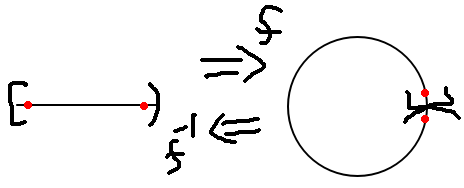
\includegraphics{1}
    \caption{Отображение $ [0, 2\pi) \to S^1 $ и обратное к нему}
    \label{fig:1}
    Точки, выделенные красным в одном случае далеко друг от друга, а в другом -- близко
\end{figure}

\begin{exmpls}
    \item $ [0, 2\pi) \to S^1, \quad S^1 = \set{(x, y) \in \R^2 | x^2 + y^2 = 1} = \set{z \in \Co | |z| = 1} $ \\
    $ f(\alpha) = \cos \alpha + i \sin \alpha $ -- непрерывно, биективно, обратное разрывно (см. рис. \ref{fig:1})
    \item $ (X, \Omega_1), (X, \Omega_2) $ -- топологические пространства (на одном множестве две топологии), $\Omega_1 \ne \Omega_2 $, $ \Omega_2 \sub \Omega_1 $ (говорят, что $\Omega_1$ -- более сильная (более тонкая) топология, чем $\Omega_2$, $f : X \to X : f(x) = x $ \\
    $ f $ -- биекция, непрерывно
\end{exmpls}

\begin{undefthm}{Чатсные примеры на $\R$}
    $ \Omega_1 $ -- дискретная, $ \Omega_2 $ -- антидискретная, $ \Omega_3 $ -- стандартная, $ \Omega_4 $ -- Зариского, $ \Omega_5 $ -- стрелка \\
    $ \Omega_1 \sub \Omega_3
    \begin{array}{c}
    	\sub \Omega_4 \\
        \sub \Omega_5
    \end{array} \sub \Omega_2 $
\end{undefthm}

\begin{note}
	$ f : X \to Y $, на $ X $ дискретная $ \implies f $ непрерывна \\
    $ f : X \to Y $, на $ Y $ антидискретная $ \implies f $ непрерывна
\end{note}

\begin{exmpls}
	\item $ (a, b) \simeq (c, d) $
    $$ f(x) = \frac{d - c}{b - a}(x - a) + c $$
    (Или любое другое непрерывное возрастающее, для которого $ f(a) = c, ~ f(b) = d $)
    \item $ (a, b) \simeq \R $ (так как $ (-\frac\pi2, \frac\pi2) \simeq \R $, через $ \tg $)
\end{exmpls}

\begin{statement}
	Гомеоморфизм -- отношение эквивалентности
\end{statement}

\begin{proof}
	\hfill
    \begin{itemize}
    	\item Рефлексивность: $ X \simeq X, \quad f(x) = x $
        \item Симметричность: $ f: X \to Y $ -- гомеоморфизм $ \implies f^{-1} : Y \to X $ -- гомеоморфизм
        \item Тринзитивность: $ f: X \to Y, g : Y \to Z $ -- гомеоморфизм $ \implies g \circ f : X \to Z $ -- гомеомрфизм
    \end{itemize}
\end{proof}

\begin{definition}
	Свойство топологического пространства называется топологическим, если оно не меняется при гомеоморфизме
\end{definition}
